%!TEX root = main.tex

\section*{Introduction}

Genetic markers have long been used in the 
management of Pacific salmon, and salmon conservation and management have been
at the forefront of a number of advances in molecular ecology,
from data generation techniques \citep{clemento2011discovery,campbell2015genotyping,mckinney2017managing}
to statistical methodology
\citep{smouse1990genetic,anderson2002model,pella2006gibbs}.
Two broadly applicable techniques that have been
actively fostered by the Pacific salmon research community are genetic
stock identification
(GSI:~\citealt{milner1982genetic,beacham2004dna,seeb2007development})
and parentage based tagging
(PBT:~\citealt{anderson2006power, garza2007large, abadia2013large, steele2013validation}).  



 In the 1980s, electrophoretically
detectable genetic variation, in the form of allozymes
\citep{ayala1972allozymes,allendorf1981use}, was used to
establish a program of GSI for Chinook salmon,
{\em Oncorhynchus tshawytscha} \citep{milner1982genetic}.  Extensive sampling
revealed that these allozyme markers
exhibited different allele frequencies among major lineages, or stocks, of Chinook salmon on the West Coast.
These allele frequency differences make GSI possible, and
\citet{milner1985genetic} soon showed that proportions of stocks in
the Washington state coastal troll fishery could be estimated by GSI.
Since that time, with the development of novel molecular markers, and, now
with increasing capacity to sequence genomic material, the scope and scale of GSI
has expanded considerably.

By using greater numbers of more variable markers than the allozymes available
in the 1980s it is possible to accurately
identify the population of origin of individual fish, rather than simply estimating
aggregated stock proportions.  It is also possible to resolve populations of fish that
are much more closely related than before.  Furthermore, reference data sets with genotypes
from hundreds of populations throughout the range of multiple species of salmon and
other anadromous species
\citep{seeb2007development,gilbey2018microsatellite,barclay2019genetic} now exist, and are routinely used to assign fish caught thousands of
kilometers from their natal streams to their stock of origin. Applications include estimating fishery
composition \citep{satterthwaite2015stock}, providing real-time information for genetics-informed fishery closures \citep{beacham2004dna}, assessing the spatial distribution of different stocks in the
ocean \citep{urawa2009stock} and their temporal distribution in upstream migrations
\citep{hess2014monitoring},  and monitoring  bycatch \citep{hasselman2016genetic} or illegal captures \citep{wilmot1999origins} in marine fisheries.

Although sequencing costs continue to decline, they are high enough
that there remains a tradeoff
between reference baselines that include information from a large number of
populations across a broad scale, and those that have been tailored
to distinguish between closely related populations on a smaller, regional scale.
Because of cost considerations, reference baselines that include populations across a broad 
spatial scale may include only a few populations from each sub-region.  Furthermore,
baselines tailored to a specific region often assemble markers that specifically
show allele frequency differences between the closely related---and hence difficult
to resolve---stocks within the region.  Consequently, regionally targeted baselines typically
outperform broad-scale baselines in resolving populations within the region.

Over the last decade an additional genetic method, parentage based tagging, or PBT,
\citep{anderson2005description,steele2019parentage}
has become established as an extremely valuable management
tool for Pacific salmon.  The availability of such family-based methods adds another factor to
consider when developing a GSI baseline.
Since the first proposal \citep{anderson2005description} to replace or augment the coded-wire tag
programme \citep{nandor2010overview}
with PBT, it has been noted that one of the major advantages of a genetic program for
PBT is that the genetic markers used for PBT could also be useful for GSI (and
vice versa).  
Thus, any panel of markers to be used for GSI (or PBT) should also be evaluated on its
utility for PBT (or GSI).

PBT has been remarkably successful in fisheries
management, having been used for over a decade in the management of Chinook salmon
and steelhead trout in major basins of the Columbia River \cite{steele2019parentage,horn2023multigeneration}, and having been employed to dramatically further our
understanding of the genetic inheritance of key traits in salmonids
\citep{abadia2013large,beulke2023distinct}. However, PBT is just one subset of a whole
family of statistical genetic methods employing relationship inference to learn about
populations.  For example inference of the full siblings amongst a sample of fish
provides information about the effective number of adults producing offspring
\citep{waples2011inbreeding,wang2023estimating}, which can
be a valuable source of information when sampling of the adults is not possible.  


Here, we present a reference baseline for Chinook salmon, targeted to the complex population 
structure within the Central Valley of California. Chinook salmon of the two main river basins---the 
Sacramento and the San Joaquin---within the Central Valley exhibit the greatest run-timing diversity
within the species.  With four recognized ecotypes, delineated primarily on the basis of run timing
(fall-, late-fall-, winter-, and spring-run), adult Chinook salmon can be found migrating or residing
in freshwater every month of the year in California. \comment{NEED MORE HERE. Certainly we should cite
\citet{yoshiyama1998historical}.}

Chinook salmon are the largest of the Pacific salmonids and have historically been the target of extremely high-value and culturally important fisheries. Moreover, because of their high degree of ecotypic variation, they have provided fishery opportunities during many different seasons and geographic locations. However, recent declines in population sizes, from the Yukon River in Arctic north, to the southern extent of their range in California has led to almost complete fishery closures  throughout most of the northeastern Pacific to protect less productive stocks. The co-occurence of fish from relatively productive and relict populations reaches its paragon in California, with the largest remaining ocean fisheries for Chinook salmon targeting the Central Valley fall-run stock that spawns in different tributaries of the same river basin as the highly endangered and phenotypically distinct winter-run stock and the threatened spring-run stocks. In spite of their distinct phenotypes and life history patterns, the four ecotypes of Chinook salmon in the Central Valley are very closely related \cite{clemento2014evaluation} and share recent common ancestry that is independent of ongoing migration between these lineages. As such, GSI has been particularly challenging in the CCV, with at least one of the distinct ecotypes, late-fall-run, unresolvable with previous GSI marker sets \cite{seeb2007development,clemento2014evaluation} and with unsatisfactory power for discriminating the protected spring-run stocks from the harvested fall-run stock.

In the following we present a new reference baseline for both GSI and PBT in California.
We describe how we identified and compiled the markers, including several new markers
that are particularly effective at distinguishing some of the closely related groups,
such as late-fall and fall-run fish.  We also provide a comprehensive analysis of this
set of markers for inference of parents and siblings within different groups of populations.



 \section*{Methods}

\subsection*{Population Sampling}

We sampled fish for the reference baselines from 13 locations within California, and one 
within Oregon. This set of populations and stocks includes all of the previously described lineages of Chinook salmon in the southern portion of the range and most of the populations that are known to have significant genetic differentiation in this region. 
These locations included sites in the two
main tributaries (the Sacramento River and the San Joaquin River) within
California's Central Valley, and the two main tributaries (Klamath and Trinity Rivers) in the Klamath basin in Northern California, and
3 rivers of the California coast (Russian, Eel, and Smith)
(Fig.~\ref{fig:map}, Table~\ref{tab:samples}).
%%%%%%%%%%%%%
\begin{figure}
\newcommand{\mapcap}{\footnotesize  A map of sampling locations represented in the reference 
baseline.  The colored circles aside
each location name represent the different run-timing groups of Chinook salmon
included in the collections from the location.  Color codes are as follows: \Wball~=~Winter run,
\LFball{}~=~Late-fall run, \Fball~=~Fall run, \Sball~=~Spring run. 
Names of each location are followed by the codes used to refer to fish from each location, with
{\tt XXF/S} indicating {\tt XXF} and {\tt XXS} are used to denote fall-run and spring-run fish
from location {\tt XX}.  Abbreviations used in location names as follows: R. = River; Ck. = Creek; H. = Hatchery; NFH = National Fish Hatchery.}
\begin{center}
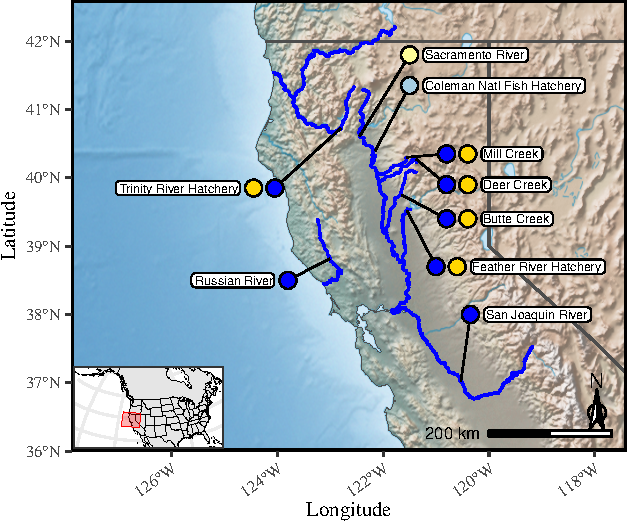
\includegraphics[width=\columnwidth]{images/map-crop.pdf}
\end{center}
\caption[\mapcap]{\mapcap}
\label{fig:map}
\end{figure}
%%%%%%%%%%%%%%%

Collections in each location were separated into fish from the different adult migration timing ecotypes according
to a variety of criteria.  Winter-run Chinook salmon are propagated at the Livingston
Stone National Fish Hatchery for supplementation (released as juveniles into the river) and as a captive broodstock;
sampling of this population was performed by hatchery staff during spawning. In Central Valley Rivers with both 
spring-run and fall-run ecotypes (i.e. Mill, Deer and Butte Creeks), previous research has documented different  (but overlapping) ranges of spawning time (Julian date) for each ecotype (\comment{REF?}).  As such, sampling targeted carcasses found in each of these 
rivers at times representative of their run-timing designation, which we were able to further confirm using their genotypes
within the region of strongest association (RoSA) on chromosome 28 \citep{thompson2020complex}. At the time of sampling (2016), only
fall-run Chinook salmon adults were found in the San Joaquin River, so the samples there were
easily categorized. Run-timing 
designation at the Feather River Hatchery is more complicated but is managed by the hatchery practices in place: 
early returning fish in May and April (expressing the spring-run life history) are visibly tagged and re-released 
to the river. Subsequently in the Fall, when hatchery raceways are reopened, only fish with the visible tag are included
as spring-run broodstock, the rest are included in the fall-run broodstock. We sampled putative spring-run and fall-run fish from these two broodstocks.  \comment{Need info about sampling in the Klamath, and on the coast}.



In total, the samples in the baseline represent fish from five different Evolutionarily Significant 
Units (ESUs) of Chinook salmon \citep{waples1991pacific}.
%%%%%%%%%%%%%%%%
\begin{table*}
\caption{\footnotesize Collections of fish in the reference baseline.  The Sampling Months column shows
a pictorial representation of the proportion of each collection sampled in each month.  Colors in
this column correspond to run-timing groups as described in the caption of Fig.~\protect\ref{fig:map}.}
\label{tab:samples}
{\footnotesize 
\begin{tabular*}{\linewidth}{@{\extracolsep{\fill}} llllllrcr}
\hline\hline\vspace*{0.4ex}
Mainstem River$^1$&Code&Location Name$^2$&Run&Reporting Unit$^4$&ESU$^4$&$N$&$N_\mathrm{day}^5$&Sampling Months&Year Range\tabularnewline
\hline Rogue R.&CRHS&Cole Rivers H.&Spring&SO-NCal-Coast&SONCC&50&0&\raisebox{-0.12 em}{
\includegraphics[height=1.02em]{../tex/images/months-CRHS_Cole-Rivers-Hatchery.pdf}}&2004--2010\tabularnewline
Smith R.&SmRF&Smith R.&Fall&SO-NCal-Coast&SONCC&46&46&\raisebox{-0.12 em}{
\includegraphics[height=1.02em]{../tex/images/months-SmRF_Smith-River.pdf}}&2010--2011\tabularnewline
Klamath R.&BCkF&Blue Ck.&Fall&SO-NCal-Coast&SONCC&56&56&\raisebox{-0.12 em}{
\includegraphics[height=1.02em]{../tex/images/months-BCkF_Blue-Creek.pdf}}&2008--2008\tabularnewline
Klamath R.&IGHF&Iron Gate H.&Fall&Klamath-Trinity&UKTR&93&92&\raisebox{-0.12 em}{
\includegraphics[height=1.02em]{../tex/images/months-IGHF_Iron-Gate-Hatchery.pdf}}&2017--2017\tabularnewline
Trinity R.&TRS&Trinity R. H.&Spring&Klamath-Trinity&UKTR&46&46&\raisebox{-0.12 em}{
\includegraphics[height=1.02em]{../tex/images/months-TRS_Trinity-River-Hatchery.pdf}}&2012--2012\tabularnewline
Trinity R.&TRF&Trinity R. H.&Fall&Klamath-Trinity&UKTR&41&41&\raisebox{-0.12 em}{
\includegraphics[height=1.02em]{../tex/images/months-TRF_Trinity-River-Hatchery.pdf}}&2012--2012\tabularnewline
Eel R.&ERF&Eel R.&Fall&Cent-Cal-Coast&CCC&93&0&\raisebox{-0.12 em}{
\includegraphics[height=1.02em]{../tex/images/months-ERF_Van-Arsdale-Fisheries-Station.pdf}}&2014--2014\tabularnewline
Russian R.&RRF&Warm Springs H.&Fall&Cent-Cal-Coast&CCC&92&92&\raisebox{-0.12 em}{
\includegraphics[height=1.02em]{../tex/images/months-RRF_Warm-Springs-Hatchery.pdf}}&2012--2012\tabularnewline
Sacramento R.&SRW&Livingston Stone NFH&Winter&CV-Winter&CVWR&111&20&\raisebox{-0.12 em}{
\includegraphics[height=1.02em]{../tex/images/months-SRW_Livingston-Stone-National-Fish-Hatchery.pdf}}&2013--2014\tabularnewline
Sacramento R.&BCS&Butte Ck.&Spring&CV-Spring&CVSR&116&116&\raisebox{-0.12 em}{
\includegraphics[height=1.02em]{../tex/images/months-BCS_Butte-Creek.pdf}}&2004--2017\tabularnewline
Sacramento R.&MDS&Deer Ck.&Spring&CV-Spring&CVSR&34&34&\raisebox{-0.12 em}{
\includegraphics[height=1.02em]{../tex/images/months-MDS_Deer-Creek.pdf}}&2002--2002\tabularnewline
Sacramento R.&MDS&Mill Ck.&Spring&CV-Spring&CVSR&50&50&\raisebox{-0.12 em}{
\includegraphics[height=1.02em]{../tex/images/months-MDS_Mill-Creek.pdf}}&2002--2004\tabularnewline
Sacramento R.&FRHS&Feather R. H.&Spring&CV-Fall&CVSR&202&202&\raisebox{-0.12 em}{
\includegraphics[height=1.02em]{../tex/images/months-FRHS_Feather-River-Hatchery.pdf}}&2010--2019\tabularnewline
Sacramento R.&FRHF&Feather R. H.&Fall&CV-Fall&CVFR&106&106&\raisebox{-0.12 em}{
\includegraphics[height=1.02em]{../tex/images/months-FRHF_Feather-River-Hatchery.pdf}}&2008--2010\tabularnewline
Sacramento R.&BCF&Butte Ck.&Fall&CV-Fall&CVFR&45&45&\raisebox{-0.12 em}{
\includegraphics[height=1.02em]{../tex/images/months-BCF_Butte-Creek.pdf}}&2004--2016\tabularnewline
Sacramento R.&MDF&Deer Ck.&Fall&CV-Fall&CVFR&24&24&\raisebox{-0.12 em}{
\includegraphics[height=1.02em]{../tex/images/months-MDF_Deer-Creek.pdf}}&2002--2004\tabularnewline
Sacramento R.&MDF&Mill Ck.&Fall&CV-Fall&CVFR&49&49&\raisebox{-0.12 em}{
\includegraphics[height=1.02em]{../tex/images/months-MDF_Mill-Creek.pdf}}&2002--2004\tabularnewline
San Joaquin R.&SJRF&San Joaquin R.&Fall&CV-Fall&CVFR&79&79&\raisebox{-0.12 em}{
\includegraphics[height=1.02em]{../tex/images/months-SJRF_San-Joaquin-River.pdf}}&2016--2016\tabularnewline
Sacramento R.&CHLF&Coleman NFH&Late-fall&CV-Late-Fall&CVFR&261&261&\raisebox{-0.12 em}{
\includegraphics[height=1.02em]{../tex/images/months-CHLF_Coleman-National-Fish-Hatchery.pdf}}&2011--2015\tabularnewline

\end{tabular*}
}
\rule{3cm}{0.3pt}

{\footnotesize
$^1$R. = River.\\
$^2$Ck. = Creek; NFH = National Fish Hatchery; R. = River; H. = Hatchery.\\
$^3$ESU = Evolutionarily Significant Unit; CVFR = Central Valley Fall Run ESU; CVSR = Central Valley Spring Run ESU; CVWR = 
Central Valley Winter Run ESU; CC = California Coastal ESU; UKTR = Upper Klamath and Trinity Rivers ESU. \\
$^4N_\mathrm{day}$: the number of samples for which the specific sampling day was recorded.
}
\hrule\vspace*{0.3ex}\hrule
\end{table*}
%%%%%%%%%%%%%%%%%%%%%

\subsection*{Genetic Markers}

We assembled genetic markers for this reference baseline dataset from several different
efforts, as detailed in the separate sections below.

\subsubsection*{Novel microhaplotype discovery}

We undertook a process to discover and validate  multiallelic
microhaplotype \citep{baetscher2018microhaplotypes} markers in California Chinook salmon, with a focus on Central Valley populations. 

We identified candidate loci with variation among multiple populations and with multiple single-nucleotide polymorphisms using reduced representation genome sequencing of 2--4 individuals each from a number of
populations ranging from California to British 
Columbia and the interior Columbia River (\comment{Table SX}).
Genomic DNA was extracted using Qiagen DNeasy 96 Blood and Tissue Kits on a BioRobot 3000 
(Qiagen, Inc). We used double-digest restriction-site associated DNA sequencing (ddRAD) and with different size selections (400 bp and 500 bp 
fragments) to produce a broad array of locus targets. Library preparation and sequencing methods followed those of
\citet{peterson2012double} with the modifications described in \citep{baetscher2018microhaplotypes}.
Sequencing was performed on a MiSeq (Illumina, Inc) using $2 \times 300$-cycle paired-end sequencing. 

Stacks v1.45 \cite{catchen2013stacks} was used to analyze ddRAD sequence data.  As there was not a well assembled Chinook salmon genome at the time, a {\em de novo} assembly was performed.  Initial filtering retained RAD loci with two or more SNPs that 
amplified in at least 10 samples. After this initial filtering, there were 3,931 RAD loci retained in the ddRAD data with 400 bp size selection and
4,794 retained in the data with 500 bp size selection. 
Gene regions were then selected that (1) contained multiple SNPs within a 100 bp window, and (2) showed haplotype variation in the winter-run 
population and at least one other.
A 100 bp window was used because the success of multiplex PCR and MiSeq sequencing is diminished in amplicons larger than 100 bp. Primer3 
software \citep{untergasser2012primer3} was used to design primers for 229 gene regions that met these criteria.  These gene regions were amplified and variants 

FreeBayes output was filtered to remove indels and retain variants with a Quality score of 30 or greater and a read depth of 10 or higher. Further filtering and analysis of the loci was conducted in MICROHAPLOT (Ng et al., DOI: 10.5281/zenodo.820110). Loci that did not conform to Mendelian segregation, that is, loci that produced more than two haplotypes within an individual were removed. Hardy-Weinberg equilibrium was assessed using MICROHAPLOT. 


\subsubsection*{Conversion of existing SNPtype assays}

A number of SNP markers from earlier discovery efforts \citep{clemento2011discovery} had already 
been validated as useful for GSI
and PBT in California \citep{clemento2014evaluation}. These markers were originally assayed
using TaqMan (Life Technologies Corp., Carlsbad, CA) probes or SNPtype assays (Standard BioTools Inc., South San Francisco, CA).
In order to type these markers using amplicon sequencing, we followed the methods in
\citet{campbell2015genotyping} and added the Illumina small RNA sequencing primer and 
read 2 sequencing primer to the SNPtype Specific Target Amplification Primer and Locus 
Specific Primers respectively.  We then dropped any loci that produced genotypes that were 
frequently inconsistent with genotypes produced with the SNPtype assays and any loci that 
did not amplify well or those that amplified so well that they were grossly over-represented
among the reads on the sequencer.  We 
used Freebayes \citep{garrison2012haplotype} to identify all variants on the fragment (not just the SNPs targeted by the original TaqMan assays).  This allows us to score each locus as a
microhaplotype \citep{baetscher2018microhaplotypes} when multiple variants occur in the sequence.  We filtered out variants
that were considered multinucleotide or complex variants by Freebayes. The resulting genetic markers are hereafter referred to as 'SNPlicons'.


\subsubsection*{Localizing markers within the genome}

The SNPlicons targets and the additional microhaplotype markers were
developed prior to the advent of a well-assembled genome for Chinook salmon.
As a consequence, many of these markers had
been used previously without certainty about their location in the genome.
After designing and validating an amplicon-sequencing approach to type both the
existing SNPtype assays and the product of the additional microhaplotype
discovery process we identified the locations of these markers within the genome by mapping the
consensus sequences (roughly 300 bp) around the markers
to both the Chinook salmon version 1 (Otsh\_v1.0; \url{https://www.ncbi.nlm.nih.gov/datasets/genome/GCF_002872995.1/}) and version 2  (Otsh\_v2.0; \url{https://www.ncbi.nlm.nih.gov/datasets/genome/GCF_018296145.1/}) genome assemblies,
using both the Burrows-Wheeler Aligner \citep{bwa-mem2009} and the BLAST-like Alignment tool \citep{kent2002blat}.
A similar mapping exercise was performed for the remaining markers so that we can
report their locations in both Otsh\_v1.0 and Otsh\_v2.0.


\subsubsection*{Identifying and Designing markers from the Late-Fall Associated Region}

To identify loci with large allele frequency differences between late-fall and fall-run Chinook salmon, 
we first conducted a simple case-control GWAS using the low-coverage whole genome sequencing 
data of \citet{thompson2020complex}, mapped to Otsh\_v1.0.  We conducted
two separate association-study comparisons.  
The first involved the 16 late-fall-run fish as cases with 16 fall-run fish from the Feather River Hatchery as controls. 
The second involved the same 16 late-fall fish as cases, but used 16 fall-run fish from the San 
Joaquin River as controls.  The association studies were performed for each chromosome with 
ANGSD \citep{pmid21663684,korneliussen_angsd_2014}, using the following command: {\footnotesize\tt angsd -yBin \{ybin\}  -r \{chrom\} 
-minMapQ 30 -minQ 20 -minInd 12 -doAsso 1 -GL 1 -doMajorMinor 1 -doMaf 1 -SNP\_pval 1e-6  
-out \{prefix\}  -bam \{bamlist\}}, where {\tt \{ybin\} } is the path to a file indicating the cases and 
controls, 
{\tt \{chrom\} } indicates the chromosome name, {\tt \{prefix\} } is the prefix to use for output files, and 
{\tt \{bamlist\} } is the path to the text file holding paths to the BAM files, one for each individual, ordered as in {\tt \{ybin\} }.

There was only one peak in association scores that was shared between both comparisons (see 
Results). From this peak we identified candidates for followup genotyping by including the 10 
SNPs with the lowest association p-values, and supplementing those with additional SNPs that 
showed:
\begin{itemize}
\item An estimated absolute allele frequency difference (between late-fall and all 32 fall-run fish)  $>0.75$,  with an approximate lower confidence interval of that figure of 0.5,  or
\item An estimated absolute frequency difference of >0.5 with a lower confidence interval >0.25 and 
with either fall-run or late-fall run being nearly fixed for one of the alleles, or
\item An annotation from snpEff \citep{cingolani2012program} of “High” or “Moderate”, or
\item An absolute frequency difference $>0.48$ and a lower confidence interval of $>0.25$ and a 
genomic  coordinate $> 2.2$~Mb.
\end{itemize}
The final condition was implemented to gather several SNPs within the flanking region to the right of 
the main peak of association. 

For the candidate markers found by the above process, we designed amplification primers using 
Primer3 \citep{koressaar2007enhancements,untergasser2012primer3} and tested amplification in a 
subset of Chinook salmon 
samples. The primer pairs that amplified sequence that reliably mapped back to the association-peak region were then typed
in a separate collection of 1,638 Sacramento River Chinook salmon sampled from the fish trap below Keswick Dam, including 1,169 winter run, 281 spring 
run, and 188 fall/late-fall run. We divided the fish identified as fall/late-fall via the 125-locus genetic 
stock identification data set into fall run and late fall run according to their sampling date at Keswick: 
99 fish arriving before Dec 26 were classified as fall run and 89 fish arriving after Dec 26 were 
classified as late-fall run.   The allele frequencies of the target SNPs at the remaining amplicons 
were 
estimated for each of these four groups: winter, spring, fall, and late-fall, and we retained
amplicons showing large allele frequency  differences between late-fall fish and all other runs.


\subsubsection*{Markers potentially associated with phenotypes \citet{thompson2020complex}}

Additionally, we include here genetic markers that characterize variation in two genes, VGLL3 and SIX6,
that have been found to be associated with phenotypes related to reproductive maturity in both
Atlantic \citep{barson2015sex} and Pacific \citep{waters2021heterogeneous} salmonids. We include
them both to provide additional variation for population genetic analyses and to
monitor populations for potential phenotypic patterns.

We include in the reference baseline amplicons targeting SNPs within the ``Region of Strongest Assocation'' (RoSA)
between spring-run and fall-run fish on Chromosome Ots28 described in \citet{thompson2020complex}.  These are useful markers to
have in the panel, as typing them routinely will create a data base for understanding the spatial and temporal
distribution of the alleles at this region; however we have omitted these markers for calculating likelihoods for
GSI, since their distribution across populations in the Feather River has been clearly and evidently
influenced by hatchery practices (see Results), and it is not necessary to include them for accurate assignment.
\comment{Describe additional E1/E2 markers (additional markers within the RoSA region) and
Tasha Marker (because it is close to the duplication noted
by Thompson et al.). We don't go into detail here---keeping it vague because it is
going to be described in the subRoSA paper, but don't mention that.}


We also include a marker that targets the sex-determining region on the Y chromosome in Chinook salmon
and that characterizes genetic sex in Central Valley populations \comment{\citep{von2015development}}


\subsection*{Amplicon sequencing and microhaplotype calling}

Amplicon sequencing was performed with the Genotyping-in-Thousands by sequencing (GT-seq) method from Campbell et al. (2015). All loci were 
multiplexed with primer concentrations ranging from 0.083 uM to 0.5 uM to increase uniformity of read depths across all loci. Sample normalization was 
performed using the SequalPrep Normalization Plate Kit (Applied Biosystems) according to the manufacturer's instructions. Samples were pooled by plate 
and then purified using Agencourt AMPure XP magnetic beads. Libraries were quantified by qPCR with the NEBNext Library Quant Kit for Illumina (New 
England BioLabs) before dilution and pooling for sequencing. All samples were sequenced on a MiSeq using $2\times 75$-cycle paired-end sequencing protocols. 
Primer sequences and concentrations for making the primer pool are in Supplemental Table 1. 

For evaluation of candidate loci, dual-barcoded sequences were used to identify individual tissue samples using the MiSeq analysis software (Illumina). The paired-end sequence reads were joined together using Fast Length Adjustment of SHort reads (FLASH: Magoc and Salzberg 2011) and mapped to an indexed sequence reference created from the Stacks target loci using BWA (Li and Durbin 2010). Mapped reads were converted to BAM files using SAMtools (Li et al. 2009) and FreeBayes (Garrison and Marth 2012) was used to call variants.

For genotyping of project samples, final filtering at each locus required a read depth of 20 and a read depth ratio of 0.30 (i.e., for heterozygotes the lower read depth haplotype must have 30\% of the total reads at that locus). MICROHAPLOT was used to call alleles and genotype processing was performed with R scripts. 

Before parentage analysis began each locus was assessed for the presence of null alleles using R scripts (eric citation). Twelve loci appeared to have null alleles in the winter-run population and were removed in all subsequent analyses. Additionally, two loci were monomorphic in the winter-run, but contained multiple alleles in other populations. The two monomorphic loci were removed in all winter-run analyses resulting in a final dataset of genotypes for 111 microhaplotype loci for this project. For more diverse salmon populations, it's likely that nearly all of the 125 microhaplotype loci could be used without Hardy-Weinberg Equilibirum or null allele issues.


\subsection*{Population genetic analyses}

Basic data summaries were calculated for each collection
using simple operations in the R programming language, Version 4.3
\citep{rcore}. We started with a simple tally of the number of alleles
found at each locus.  To provide a summary of the genetic variation and
missing data we report:
\begin {itemize}
\item the average over loci of the number of fish
in which each locus was successfully genotyped, $\bar{N}$;
\item the average number of alleles per locus in each collection with all collections
downsampled to the smallest number of genotyped individuals at each
locus, $\bar{N}_\mathrm{A,ss}$;
\item the fraction of polymorphic
loci in each collection after subsampling to the smallest number of genotyped
fish, $\bar{P}_\mathrm{poly,ss}$;
\item the expected heterozygosity as the average over loci
of one minus the frequencies of homozygotes at each locus expected from the
estimated allele frequencies, $\bar{H}_\mathrm{exp}$; and 
\item the observed heterozygosity as the average over
loci of the fraction of heterozygous genotypes, $\bar{H}_\mathrm{obs}$.
\end{itemize}
When subsampling each collection to the minimum number of genotyped
fish across all collections at a locus, we subsampled individuals without
replacement, taking the average of 1,000 different random subsamples.  

We calculated \citet{weir1984estimating}'s pairwise $F_\mathrm{ST}$ between
all collections, using the {\footnotesize\tt pp.fst} function from the R
package 'hierfstat' \citep{hierfstat}. Finally, we evaluated population
structure in the data by performing unsupervised clustering of
the complete data set
using the program STRUCTURE \citep{pritchard2000inference,falush2003inference}.
We performed 20 replicate runs at each value of the assumed number of
subpopulations, $K$, in $\{2, 3, 4, 5, 6, 7\}$ 
using default settings of the program.  STRUCTURE output was
a summarized and visualized using CLUMPAK version~\comment{??}
\citep{kopelman2015clumpak}.






\subsection*{Power for genetic stock identification and population assignment}

To assess the power of the marker panel for GSI, we used the R package
'rubias' \citep{moran2019bayesian}.  We used the function {\tt self\_assign()}
to perform assignment of each individual in the reference baseline to one of the
collections within the baseline.  Each fish was removed from the reference baseline
when calculating the likelihood that it originated from the collection it actually belongs
to, using a classical leave-one-out approach to eliminate the inflated estimates of
power that might occur without such a procedure \citep{anderson2008improved}.
The scaled likelihoods of collection membership returned by
{\tt self\_assign()} were summed within reporting units, and fish were
assigned to the reporting unit with the largest value of that sum.  Subsequently,
fish were assigned to the collection within that reporting unit with the highest
scaled likelihood.  We considered two criteria for assignment.  In the first,
all fish are assigned, in the second only fish with a summed (i.e., summed
over all collections in a reporting unit)
scaled likelihood greater than 0.8 were assigned.

Finally, we investigated the matrix of assignments and misassignments
broken down according to the genotype of the fish at the markers within
the RoSA.  For this, \comment{Eric. Describe this from what you have in the notebook}. 


\subsection*{Power for relationship inference}

To explore the utility of the marker panel for relationship inference, we used
the R package `CKMRsim'
(\url{https://github.com/eriqande/CKMRsim})
to estimate the false-positive rates (FPRs) expected at
different values of the false negative rate (FNR) for a variety of different pairwise
relationships in different populations.  For these purposes, we divided the
collections into 10 different groups.  The members of each group are
relatively similar For all cases, we assumed that the genotyping error rate
was 1\% per locus and the genotyping error model was the default
"True-genotype-independent" model. 

For errors involving misidentifying
unrelated (U) pairs as parent-offspring (PO), full-sibling (FS), or half-sibling (HS)
pairs we used importance sampling to estimate the very small FPRs.  The
FNRs were estimated in each case using simple Monte Carlo.  For the FS and
HS cases the FNRs were calculated from Monte Carlo sampling while taking account
of the physical linkage of the markers by inputting their genomic positions into
'CKMRsim' and using the MENDEL \citep{lange2013mendel} software to simulate genotypes of related pairs
in the presence of physical linkage.  For PO pairs (and U pairs),
FNRs were calculated without reference to the genomic locations of the markers
because physical linkage does not
affect the distribution of log-likelihood ratios in those two relationship types,
because there is no variation, anywhere
in the genome, in the number of gene copies shared identical by descent between
a parent and its child or between two unrelated individuals.

For errors involving misidentifications between the relationship
types of avuncular (AN: aunt-niece, uncle-nephew, etc.), PO, FS, and HS,
we used regular Monte Carlo to estimate the FPRs and FNRs, because
importance sampling cannot be used in those cases, and, since there are
expected to be far fewer such relationships than the number of unrelated
pairs expected, the relevant FPRs are not so tiny and can be estimated
(at least down to rates of $10^{-3}$) reliably.  For AN, FS, and HS, both the
FPRs and FNRs were estimated while taking account of physical linkage
of the markers, as described above.

\section*{Results}

\subsection*{Genetic Markers}

\subsubsection*{Conversion of existing SNPtype assays}

Of the 96 existing SNPtype assays, we were able to convert 79
into reliable amplicon-sequenced assays that were included in the panel.

\subsubsection*{Additional microhaplotype discovery} 

We tested 229 candidates from our additional microhaplotype discovery and
initially retained the 125 markers described in \citep{thompson2020complex}
for use in stock identification within
the Klamath Basin.  However, further evaluation of those markers in other
populations led us to drop some, and retain 106 of those markers in the current panel.

\subsubsection*{Localizing markers within the genome}

Of these \comment{185} loci that originated from SNPtype assays or from our additional
microhaplotype discovery, \comment{179} of them mapped identically to a single
location on an assembled chromosome in the Otsh\_v2.0 genome, using both bwa mem and BLAT.
Of the remaining 6 loci, one of them was mapped to the same location by BLAT and bwa mem, but
the alignments differed by one base pair in the length of an embedded insertion, two of them had a single secondary alignment on a different chromosome
that was identical in both bwa mem and BLAT, two of them had secondary alignments that
disagreed slightly between BLAT and bwa mem, and one of them had multiple
non-primary alignments (Table~S1 \comment{This is the Excel File.  It needs to
be edited so as to: 1) have a column
giving the category or provenance of the markers (i.e. LFAR or MHAP or SNPTYPE, etc.) 2) retain
only the 2 LFAR markers we actually use. 3) Definitely rename the E2 markers to be something other
than winter-run-greb1L-diagnostic}).

Mapping to Otsh\_v1.0 was similar, except that a greater number of markers mapped to unplaced
scaffolds in Otsh\_v1.0 than in Otsh\_v2.0, likely reflecting the more complete nature of the
second assembly.  

\subsubsection*{Late-fall Associated Region Markers}

The case-control association test revealed a single peak on chromosome 34 with large allele frequency differences
between Central Valley late-fall and fall-run fish.  This peak was evident both in the comparison of
late-fall fish to fall-run fish in the Feather River Hatchery and of late-fall fish to the fall-run fish in
the San Joaquin River (Fig.~\ref{fig:lfar-assoc}).




The Manhattan plot of Fig.~\ref{fig:lfar-assoc} shows sporadic SNPs with low association
$p$-values.  These are not shared between the two different late-fall to fall comparisons, and
sites that we investigated were concentrated in areas of poor mapping suggesting that their
$p$-values were artifactual.  By contrast, a large number of sites near the prominent peak on
chromosome 34 had large allele frequency differences between late-fall and fall run.  Taking the
10 SNPs with the lowest association $p$-values, and including additional ones from the filtering criteria given in the
Methods, yielded 49 candidate markers for which we designed primers for amplication.  Only 8
of these 49 primer pairs yielded reliable amplification and mapping.   Of these 8, two of the SNPs 
showed inconsistent genotyping and were removed from consideration.  Of the remaining 6, only 3 
showed marked allele frequency differences ($> 0.7$) between late-fall and fall run.  These three 
SNPs (located at: Chr34:828,768,  Chr34:865,057, and Chr34:1,063,084 in the Otsh\_v1.0 assembly)
also had pronounced differences in allele frequency between 
late-fall and spring or winter run.

Analysis of the mapping of amplicons for Chr34:828,768 
showed that many ($\approx$89\%) of the reads were off-target (aligning to other chromosomes, 
etc.), making it costly (in terms of sequencing effort) to include the marker in the baseline panel. 
\comment{Consequently it was dropped.}  The frequency of the different alleles at the two remaining loci
within different reporting units in the baseline are shown in Table~\ref{tab:lfar-freqs}.
%%%%%%%%%%%%%%
\begin{table}
\caption{\footnotesize Allele frequencies across reporting units of the two late-fall associated
markers.  Frequencies are given for the alleles most common amongst late-fall Chinook: nucleotide 
{\tt G} at locus Chr34:865,057 and {\tt A} at Chr34:1,063,084.  $N$ is the total number of gene 
copies available for estimating the allele frequency.}
\label{tab:lfar-freqs}
{\footnotesize
\begin{tabular*}{\columnwidth}{@{\extracolsep{\fill}} lrrrr}
\hline\hline
& \multicolumn{2}{c}{\underline{Chr34:865,057}} & \multicolumn{2}{c}{\underline{Chr34:1,063,084}} \\
Reporting Unit & freq. & $N$ & freq. & $N$ \\ \hline
CV-Late-Fall&0.750&516&0.733&592\tabularnewline
CV-Fall&0.054&910&0.030&908\tabularnewline
CV-Spring&0.023&396&0.003&396\tabularnewline
CV-Winter&0.005&222&0.005&222\tabularnewline
Cent. Cal. Coast&0.000&92&0.004&278\tabularnewline
Klamath-Trinity&0.000&172&0.000&358\tabularnewline
SO-Ncal-Coast&0.000&192&0.000&304\tabularnewline

\end{tabular*}
}
\vspace*{-2.3ex}\hrule\vspace*{0.3ex}\hrule
\end{table}
%%%%%%%%%%%%%%%
\subsection*{Population genetic summaries}

The total number of alleles per locus varied between 2 and 10 (Fig.~\ref{fig:num-alle}). Biallelic 
loci were most common, at 66 of the total, but two-thirds of the microhaplotype markers
showed more than two alleles, which has been shown to provide significantly more
power for relationship inference than a comparably sized panel of biallelic SNPs
\citep{baetscher2018microhaplotypes}.


The population-genetic summary statistics are presented in Table~\ref{tab:pg-summ}.
%%%%%%%%%%%%%%
\begin{table}
\caption{\footnotesize Simple population genetic summaries. All quantities are means
over loci.  $\bar{N}$ is the number of fish with observed genotypes; $\bar{N}_\mathrm{A,ss}$ is the
average number of alleles and $\bar{P}_\mathrm{poly,ss}$ the fraction of polymorphic loci,
after sub-sampling to the smallest sample size per locus; $\bar{H}_\mathrm{exp}$ and
$\bar{H}_\mathrm{obs}$ are expected and observed heterozygosity, respectively. Population
codes are as given in Table~\ref{tab:samples}}
\label{tab:pg-summ}
{\footnotesize
\begin{tabular*}{\columnwidth}{@{\extracolsep{\fill}} lrrrrr}
\hline\hline
Code&$M$&$\bar{N}_\mathrm{A,ss}$&$\bar{P}_\mathrm{poly,ss}$&$\bar{\mathrm{H}}_\mathrm{exp}$&$\bar{\mathrm{H}}_\mathrm{obs}$\tabularnewline
\hline CRHS&0.008&2.60&0.95&0.398&0.399\tabularnewline
SmRF&0.021&2.60&0.95&0.401&0.394\tabularnewline
BCkF&0.041&2.59&0.96&0.393&0.382\tabularnewline
IGHF&0.028&2.37&0.93&0.356&0.363\tabularnewline
TRS&0.036&2.37&0.92&0.353&0.348\tabularnewline
TRF&0.031&2.37&0.92&0.352&0.351\tabularnewline
ERF&0.022&2.51&0.95&0.364&0.356\tabularnewline
RRF&0.037&2.64&0.96&0.398&0.391\tabularnewline
SRW&0.338&2.32&0.88&0.338&0.329\tabularnewline
BCS&0.046&2.52&0.92&0.379&0.373\tabularnewline
MDS&0.082&2.55&0.94&0.394&0.397\tabularnewline
FRHS&0.108&2.61&0.95&0.397&0.392\tabularnewline
FRHF&0.029&2.63&0.96&0.394&0.398\tabularnewline
BCF&0.123&2.60&0.94&0.385&0.370\tabularnewline
MDF&0.130&2.59&0.94&0.386&0.383\tabularnewline
SJRF&0.012&2.57&0.94&0.384&0.380\tabularnewline
CHLF&0.068&2.53&0.94&0.386&0.384\tabularnewline

\end{tabular*}
}
\vspace*{-2.3ex}\hrule\vspace*{0.3ex}\hrule
\end{table}
%%%%%%%%%%%%%%%
The average number of fish with non-missing data in each population varied from
a low of 39.2 (BCF) to a high of 275.2 (CHLF).  The average number of alleles
per locus, standardized to the smallest sample size, ranged from 2.35 (SRW) to
2.68 (RRF), with  SRW also having the smallest value of the
standardized fraction of polymorphic markers at 0.9 and RRF sharing the highest value
(0.97) with ERF and BCkF.
SRW also had the lowest values for expected and observed heterozygosity:
0.349 and 0.340, respectively. While the highest for expected heterozygosity
was 0.412 (SmRF) and for observed heterozygosity, 0.411 (CRHS).

The estimated pairwise $F_\mathrm{ST}$ values between the collections
varied from a low of 0.0 to a high of 0.273 (Figure~\ref{fig:gsi}a).
Notably, most of the largest values
of $F_\mathrm{ST}$ occurred between SRW and another collection.  

The program STRUCTURE clustered fish at all values of $K$ from 2 to \comment{7}.
(Fig.~\ref{fig:struct}).  The clusters generally corresponded to groupings of related populations, and confirmed
{\em a priori} knowledge about which collections in the baseline could and should be
grouped together into reporting units.  At every value of $K$ CLUMPAK discerned at least
11 of 20 replicates in the major mode (Fig.~\ref{fig:struct}). Clustering solutions in the minor
modes appear in Fig.~\ref{fig:minor-modes}.
%%%%%%%%%%%%%%%%%%%%
\begin{figure}
\newcommand{\structcap}{\footnotesize Major modes found by STRUCTURE and summarized
by CLUMPAK out of 20 replicates for each value of $K$, the assumed number of
subpopulations. \comment{We kind of need to make our own figure here that doesn't take up
as much whitespace and also gives the number of occurrences of each mode.} }
\begin{center}
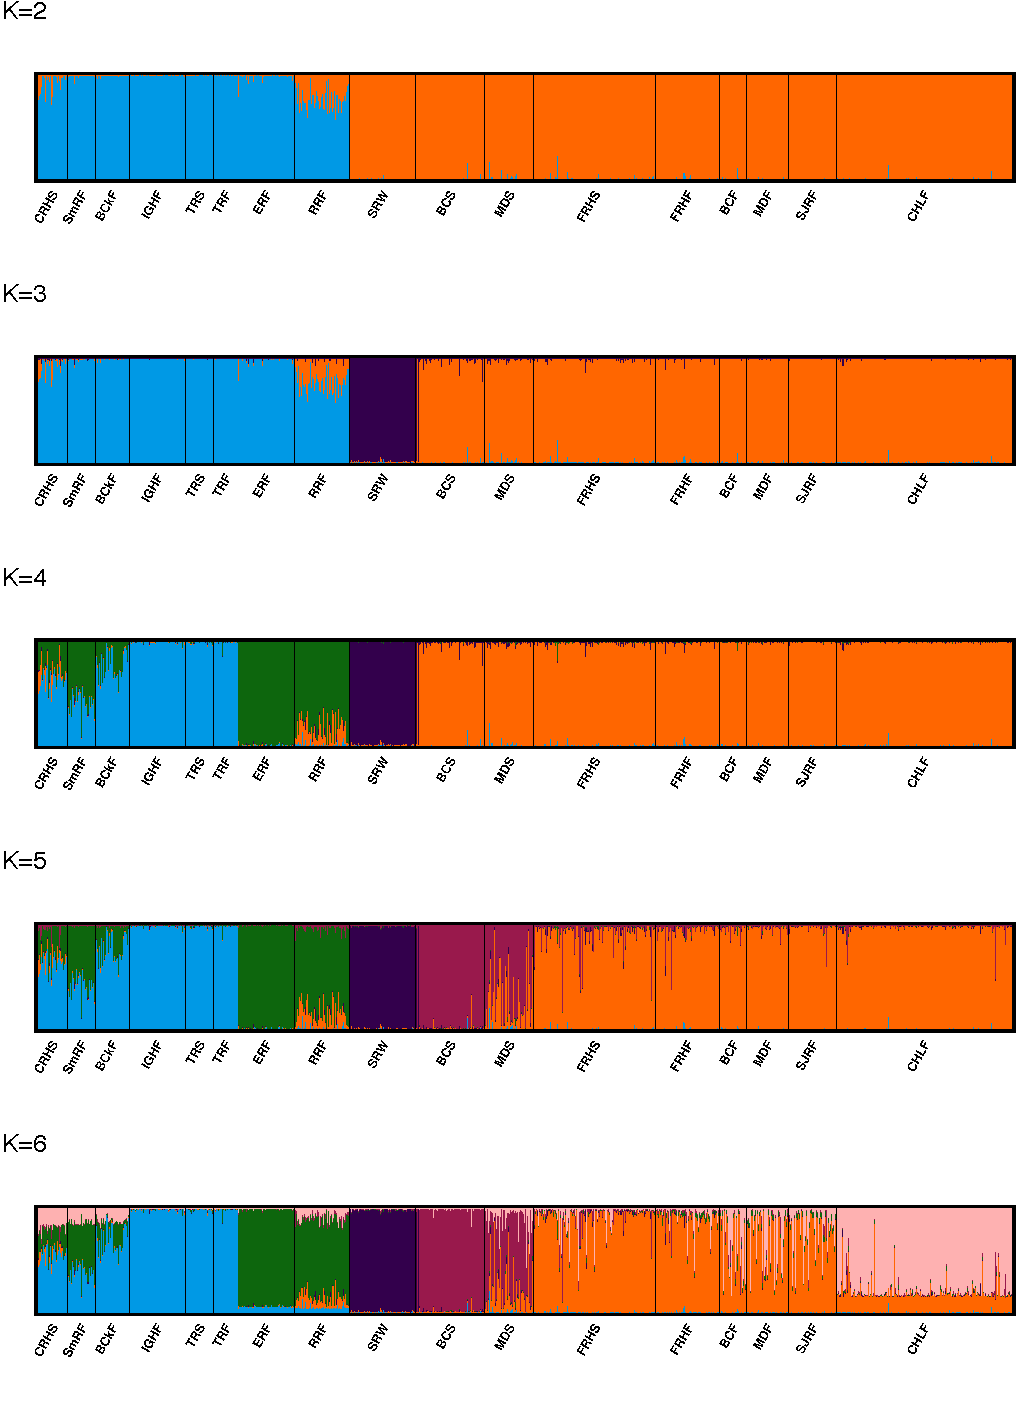
\includegraphics[width=\columnwidth]{images/major-modes-crop.pdf}
\end{center}
\caption[\structcap]{\structcap}
\label{fig:struct}
\end{figure}

\subsection*{Power for genetic stock identification and population assignment}

Leave-one-out cross-validation (self-assignment) analysis demonstrates that this
reference baseline provides a high degree of accuracy for distinguishing the major
groups of Chinook salmon in California.  The results of the analysis are summarized
in a self-assignment matrix (Figure~\ref{fig:gsi}). 
%%%%%%%%%%%%%%%%%%%%%% 
\begin{figure}
\newcommand{\gsicap}{\footnotesize Pairwise $F_\mathrm{ST}$ values and allele frequencies({\bf a)} 
and self-assignment rates
 ({\bf b)}  for the collections in the baseline.  The codes of the populations
appear on the outer margins of the table atop cells colored according to the run-timing group
of the collection.  Interior cells in which the column and row correspond to the same reporting
unit are colored according to the reporting unit.  In ({\bf a}), for $F_\mathrm{ST}$ values, the upper triangle was computed using the baseline microhaplotype
data. Each cell in the lower triangle shows a small scatter plot of estimated allele frequencies
in the collections---the $x$ value is allele frequencies from the collection in the column and the
$y$ value is from the collection in the row. Frequencies for all alleles are shown, with values within
each cell ranging from 0 to 1.  These frequencies were estimated by, for each locus, randomly
subsampling individuals from each collection to the minimum number of observed alleles in any collection
at the locus.  In ({\bf b}), for self-assignment tallies, the row corresponds
to the true source collection and the column corresponds to the assigned collection.
\comment{Hey! Didn't we drop one of the LFARs? I see three, still.}}
\begin{center}
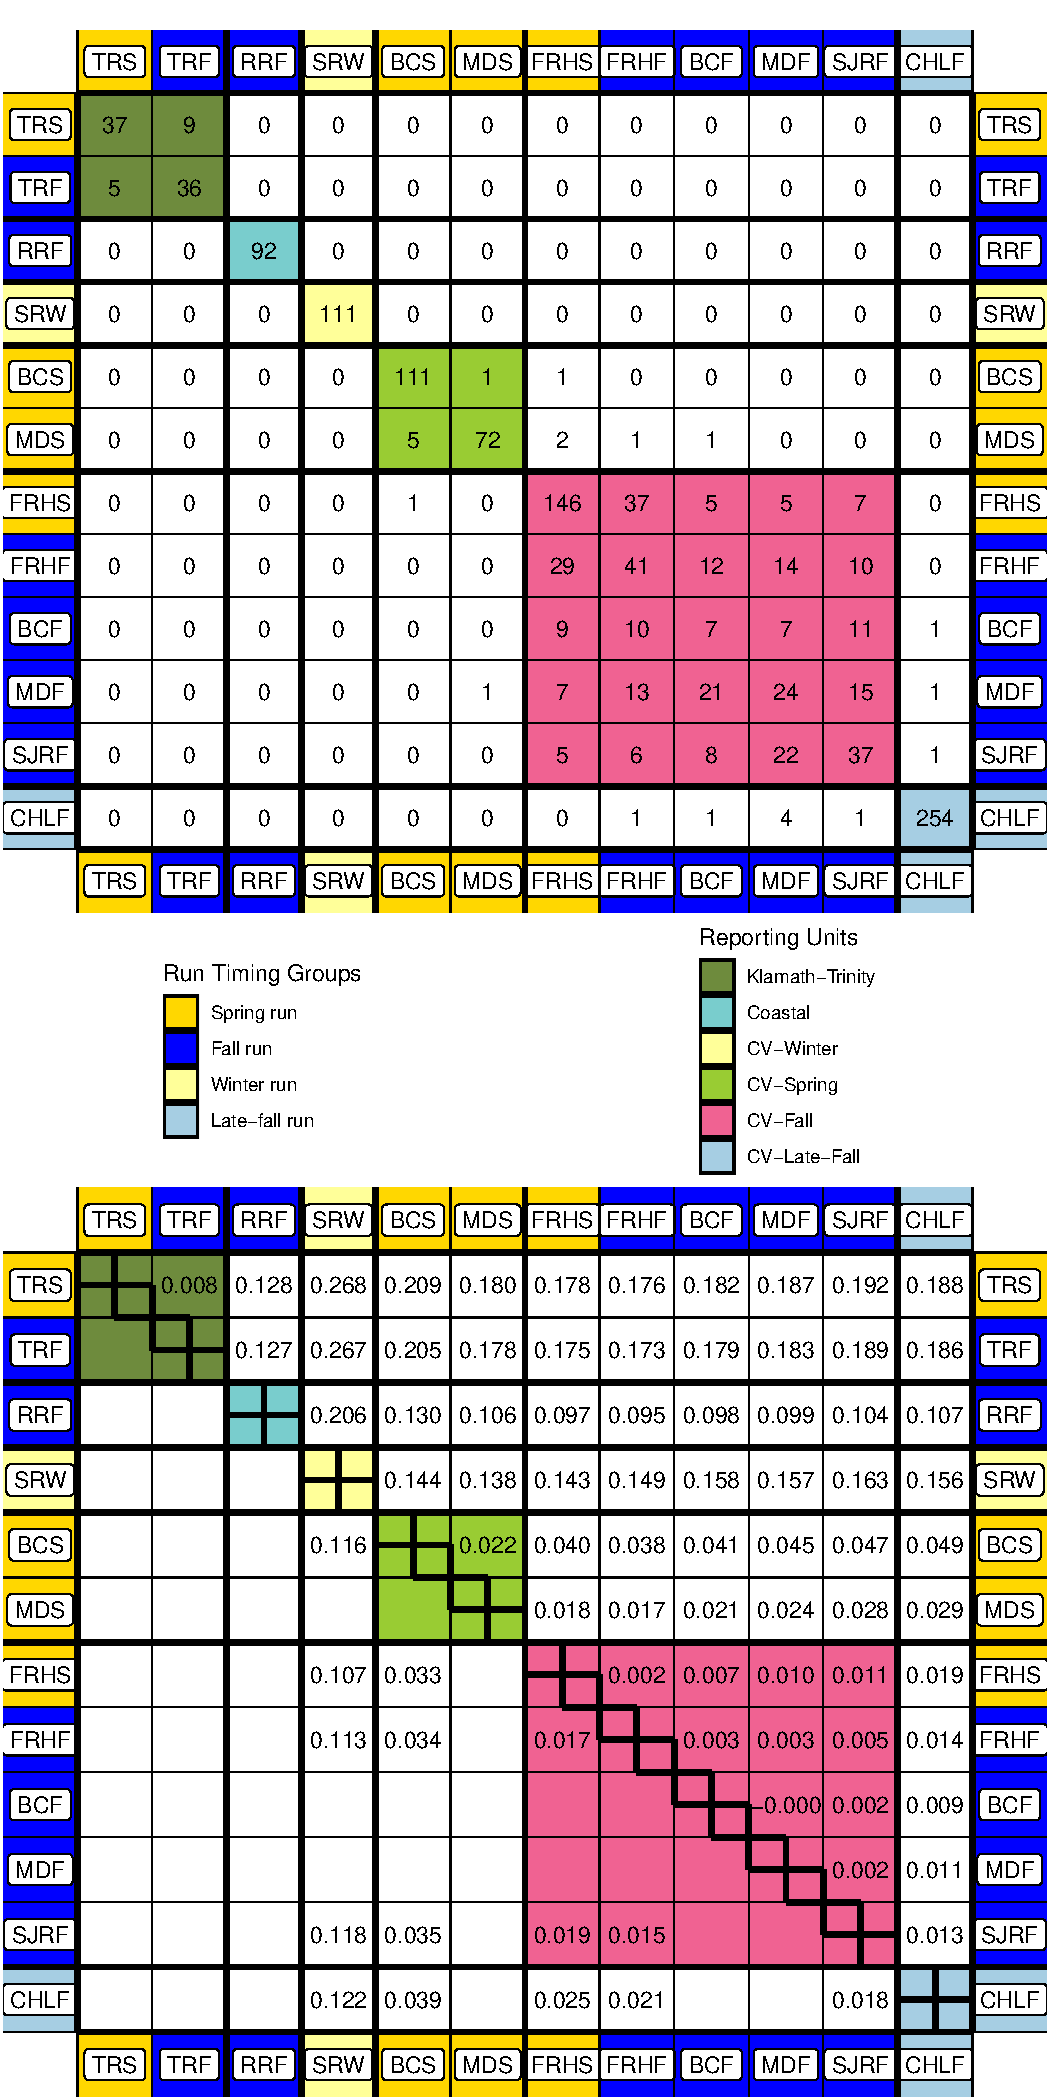
\includegraphics[width=\columnwidth]{images/gsi_and_fst_fig-crop.pdf}
\end{center}
\caption[\gsicap]{\gsicap}
\label{fig:gsi}
\end{figure}
%%%%%%%%%%%%%%%%%%%%
This figure shows the collections divided into seven different reporting groups:
SO-Ncal-Coast,  Klamath-Trinity, Cent. Cal. Coast,
CV-Winter, CV-Spring, CV-Fall, and  CV-Late-Fall.  \comment{Really, where and how
do we want to introduce these reporting units?} These groupings correspond
largely to the divisions in the data found by STRUCTURE, and they also correspond
with divisions amongst the stocks as defined for management.

Overall, of the 1613 fish in the reference baseline, 1587 (98.4\%) were correctly
assigned to their reporting unit of origin, while 26 (1.6\%) were incorrectly assigned.
Four of those 26 misassignments which involved fish being incorrectly assigned to
SRW, were clearly fish from SRW that had been incorrectly sampled into a different
collection, likely due to straying. (This is evident because SRW are so distinct that it is not possible
to incorrectly identify them).  Of the remaining 22 misassignments,  9 involved fish from the
CHLF (late fall run) collection being misassigned to the CV-Fall reporting unit and 7 were
fish from the MDS (Mill-Deer spring run) collection being assigned to the CV-Fall reporting unit.
It is possible that some of these misassignments represent CV-Fall fish that were incorrectly
sampled as CHLF or MDS; however, unlike with SRW, that we could not conclude that
confidently, as there is some degree of overlap in likelihood values between the two.

While fish from CHLF were found to misassign at a rate of 3.1\% (9/291) and MDS at a rate 
of 8.6\% (7/81) to CV-Fall, are seen to misassign at fairly high rates to CV-Fall, the
converse is not evident---that is, fish from the CV-Fall are misassigned to CHLF at a rate
of only 0.6\% (3/501) and to the CV-Spring reporting unit (to which MDS belongs) at a rate
of only 0.4\% (2/501).  

When assignments are only accepted with a scaled likelihood greater than 0.8,
18 assignments are discarded, but not all of those were incorrect.  At the 0.8 threshold,
the total fraction of correct assignments is 98.8\% (Fig.~\ref{fig:eighty}).

We note that the RoSA markers provide the differential signal necessary to distinguish the
Feather River spring-run stock from the other CCV stocks with a predominantly fall-run
genomic background, as they do not share genome-wide ancestry with the other spring-run
stocks/lineages in the basin. In this context, it is clear that the 'fall-run' hatchery
program in the Feather River both spawns and produces many spring-run fish and RoSA heterozygotes.
Similarly, in other regions, the RoSA markers are the only way to distinguish fall-
and spring-run fish, as they otherwise share genomic background. 
In California, only the Sacramento and  Klamath basins have documented spring-run
salmon and their historical occurrence in other basins has been unclear. We find no
instance of spring-run fish in these coastal basins, but did identify one copy of the early-lineage
RoSA haplotype in the Eel River. Moreover, we identified three additional copies of a
recombinant haplotype that carries half of the RoSA SNPs from both the E and L lineages in the Eel and Russian rivers. No other clear recombinants were identified in the study populations, indicated that it arose in the California Coastal Chinook Salmon lineage, and provides further evidence of past presence of RoSA haplotypes associated with early migration.





\subsection*{Power for relationship inference}

The results are summarized in Fig.~\ref{fig:fprs}.
%%%%%%%%%%%%%%%%%%%%%
\begin{figure*}
\newcommand{\fprcap}{\footnotesize False positive rates (FPRs) as a function of false negative
rates (FNRs) for distinguishing between different relationships.  {\bf (a)} FPRs calculated
using importance sampling of unrelated pairs of individuals being incorrectly categorized as parent-offspring (PO),
full-sibling (FS) or half-sibling (HS) pairs.  {\bf (b)}  FPRs calculated using regular Monte Carlo
sampling of avuncular pairs (AN: aunt-niece, uncle-nephew, etc.) or full-siblings (FS) or half-siblings (HS) being 
incorrectly categorized as parent-offspring (PO); as well as FPRs of parent-offspring (PO) pairs or half-sibling (HS) 
pairs being incorrectly inferred as full siblings (FS).  In both {\em a} and {\em b}, 100,000 Monte Carlo replicates 
were simulated.  Importance sampling allows estimation of very small false positive rates for unrelated pairs, but 
cannot be applied to truly related pairs.  Consequently, it is difficult to accurately estimate small probabilities 
($10^{-4}$ or less) in {\bf b}, as indicated by the error bars, which represent the estimate $\pm 2s$ where $s$
is the estimated standard error of the mean of the Monte Carlo sample.  This also is the reason that many of the lines terminate.   }
\begin{center}
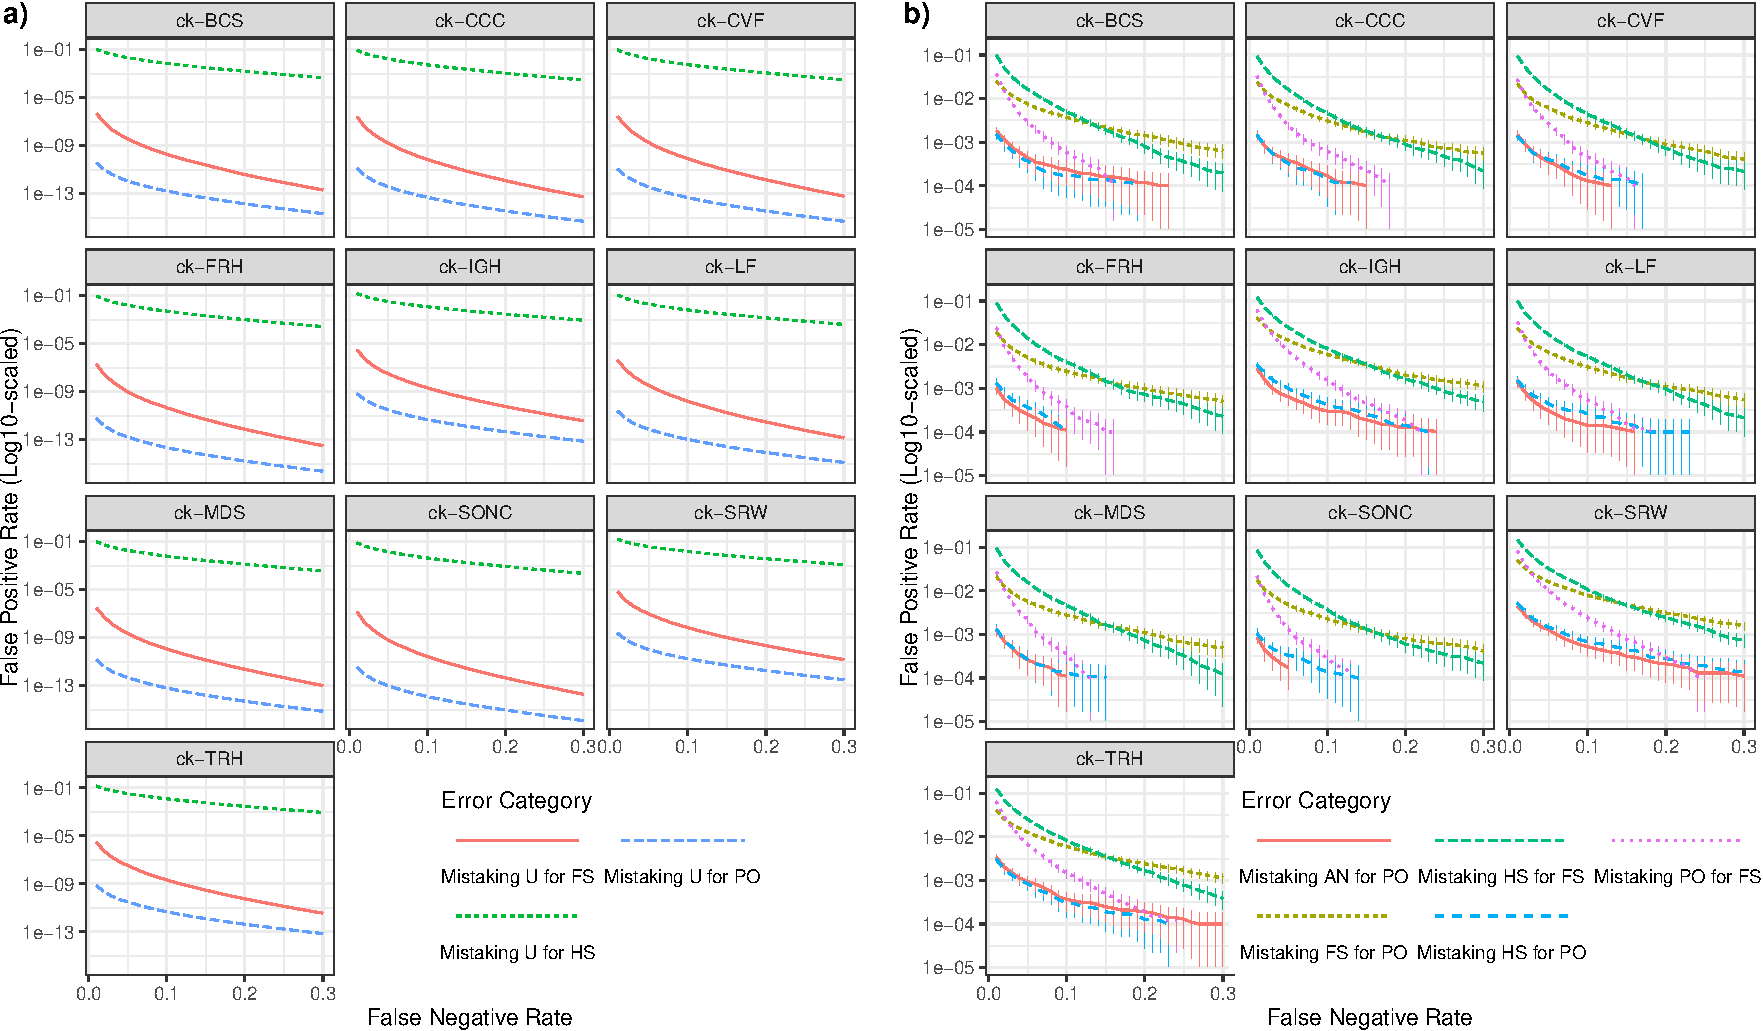
\includegraphics[width=\textwidth]{images/fpr-fnr-figure-crop.pdf}
\end{center}
\caption[\fprcap]{\fprcap}
\label{fig:fprs}
\end{figure*}
%%%%%%%%%%%%%%%%%%%%
And we can also point readers to the supplement figure \ref{fig:ckmr-comp}.
The power analyses for this set of markers demonstrate that they have ample variation
for accurate identification of parent-offspring (PO) and full-sibling (FS) pairs in almost all
realistic situations. The predicted false positive rates for both PO and FS pairs are
exceedingly low for even stringent false negative thresholds (e.g. 0.05). 
For example, the false positive rate for FS identification is less than one error in 10 million
comparisons of potential siblings in the California Chinook salmon population with the lowest
heterozygosity (SRW) at a false negative rate of 0.05. However, HS pairs can not be accurately
distinguished from unrelated pairs in any populations without very large false negative rates
and in very modest-sized studies.
We note, however, that the presence in a dataset of genotypes from individuals that are related, but not in
 the relationship category proposed, will result in some additional misidentifications.
 These 'errors' will all involve related fish being identified as such, but in the incorrect relationship category.  The cross-assignment frequencies predicted for some common relationship categories, and for realistic FPR and FNR, are found in (Fig 4b).


 
\textbf{Although some additional errors might be
expected when related but non-FS individuals are sampled,  this number of comparisons exceeds
those necessary in almost all realistic scenarios.
We note that, as in previous work, it is nearly impossible to identify HS pairs accurately
with data from this, or any standard marker dataset. However, the use of properly LD-filtered
genome-scale data should allow such discrimination in future work.
Accurate relationship
inference in even the most genetically depauperate Chinook salmon population in California
and rangewide (Seeb et al. 2007, Clemento et al. 2014) is therefore possible with this marker set.}


While there is not a currently available method (like that of \citeauthor{anderson2006power}) for estimating error rates in
inference of parent-offspring trios with multiallelic marker data, given the substantial amount of statistical power for identifying PO and FS pairs, which require much more statistical power, it is clear that PO-trio inference with these markers will be essentially error free.



\section*{Discussion}

We describe a novel panel of microhaplotype genetic markers for Chinook salmon 
in California that includes multiallelic gene regions with high variability for 
relationship inference and gene regions identified in whole-genome sequence data 
for increased power for population identification. We show how this set of markers
provides sufficient power for highly accurate identification of parent and offspring
pairs and full siblings in California Chinook salmon, and also allows near-perfect 
identification of individuals to population or genetic group of origin. This set of 
genetic markers lays the foundation for a comprehensive genetic monitoring and evaluation effort
that facilitates multiple types of inference and is flexible and extensible.
When, and if, sequencing costs drop sufficiently, it may be possible to include
all different populations of a single species within a single standardized reference baseline
that performs equally well at broad and regional scales. A statistical approach for population
assignment from low coverage whole genome sequences appeared recently
\citep{desaixINPRESSpopulation}, and its authors noted that such a data type could
be ideal for producing reference baselines simultaneously applicable to broad scale
coverage and high resolution within sub-regions.   For the present, however,
baselines tailored to specific regions are essential for regional management questions.

Although previous work using genome-scale data has shown that many of these populations or stocks can be resolved \cite{thompson2020complex,meek2020identifying},
such data is not practical for most large-scale applications of GSI and PBT, particularly because
of the much higher costs, longer turnaround time and challenges of producing highly
replicable datasets with reduced representation and low-coverage whole genome sequencing methods \cite{ali2016rad}. 
Accurate identification of the distinct ecotypes of Chinook salmon in the California Central Valley is of utmost importance for designing and implementing effective conservation and management actions. This has been challenging, given the recent common ancestors of these ecotypes and ongoing migration between subbasins. We describe the first set of genetic markers that identifies the late-fall-run salmon ecotype, which occurs only in the CCV and shares a genomic background with the more common CCV fall-run salmon ecotype. Moreover, we show how the FRH spring-run lineage is easily identifiable through a combination of traditional GSI and the characterization of functional genetic markers in the RoSA. Finally, although previous work has described GSI capabilities that distinguish the natural-spawning CCV spring-run lineages from each other and their fall-run counterparts with moderately high accuracy, we demonstrate near complete accuracy in distinguishing these 'stocks'. Moreover, the few fish that are apparently misidentified (Fig. 3) are likely to be primarily migrants and not true misidentifications. For example, the three fish that were field-characterized as spring-run from Butte Creek, but are genetically identified as winter-run salmon are clearly carry the winter-run genomic background and could not realistically be misidentified on the basis of the genetic data. This marker set and baseline reference dataset also provides unprecedented power for identifying fish from not only the other ESUs in California, but even the individual populations within those ESUs (Fig. 3).
Additionally, previous genetic marker sets for California Chinook salmon had sufficient power for inferring parent-offspring relationships, but only when both parents were sampled and genotyped. This marker set considerably increases the capacity for relationship inference in California salmon, by providing sufficient power for parent-offspring relationship inference, when only one parent was sampled, as well as identifying pairs of full siblings when no parents are sampled. Groups of full siblings larger than two are identified even more accurately than expressed in Figure 4. 

